\documentclass[12pt]{article}

% The preceding line is only needed to identify funding in the first footnote. If that is unneeded, please comment it out.
\usepackage{cite}
\usepackage{amsmath,amssymb,amsfonts}
\usepackage{algorithm}
\usepackage{algorithmic}
\usepackage{graphicx}
\usepackage{textcomp}
\usepackage{xcolor}
\usepackage{colortbl}
\usepackage{float}
\usepackage{subcaption}
\usepackage{multirow}

\def\BibTeX{{\rm B\kern-.05em{\sc i\kern-.025em b}\kern-.08em
    T\kern-.1667em\lower.7ex\hbox{E}\kern-.125emX}}
\begin{document}

\title{Coursework of Neural information Processing cousework}



\author{Chen Ting Hung} {}
	
\maketitle

\begin{abstract}
This is the report of out Neural information Processing cousework
\end{abstract}

\section{Question 1}
How does the algorithm work? Plot the different components of the algorithm over learning to help you explain its behaviour (e.g. what are the weight changes given by backprop, how do the different components of TD-learning change as the agent explores the environment, or/and plot the features/weights at different points during learning). You should also plot the performance of the algorithm over the learning iterations (i.e. the learning curve).\\

Answer1:\\
Backpropagation algorithm is divided into two parts first is feedforward and second backforward part \\
when we doing backforward part we will update two side of weights and bias one is input to hidden layer and seconde is hidden layer to output layer.\\
And after lots of times traning the model which backpropagation algorithm learn become more precisely.\\
In this coursework we also implemented sigmoid function as an activate function and we just only use one hidden layer.\\
The reason is that it would be more easier.

In following picture it shows that how bias update in different iterations.\\
It is present that the bias value decrease in the beginning. After reach the lowest point it raise agian. Finally, it's value arise agian and then we get the best value around 3 to find the best value.\\
The second picture is showing the loss function. It is trying to compare with the output from this model and the truth value.\\
It is obvious that to see that loss function decrease sharply around 10000 times and the result become more precise.
\begin{figure}[htb]
    \centering
    \begin{subfigure}[b]{.48\linewidth}
    \centering
    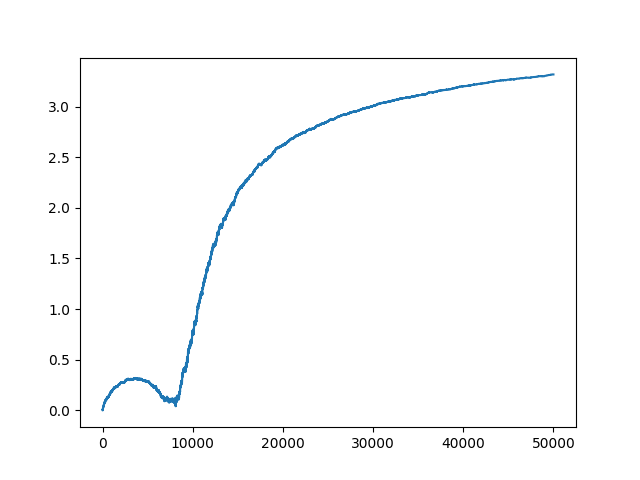
\includegraphics[width=\linewidth]{bias.png}
    \caption{\textbf{\texttt{bias.jpg}}}
    \end{subfigure}
    \label{fig:1}
    \begin{subfigure}[b]{.48\linewidth}
    \centering
    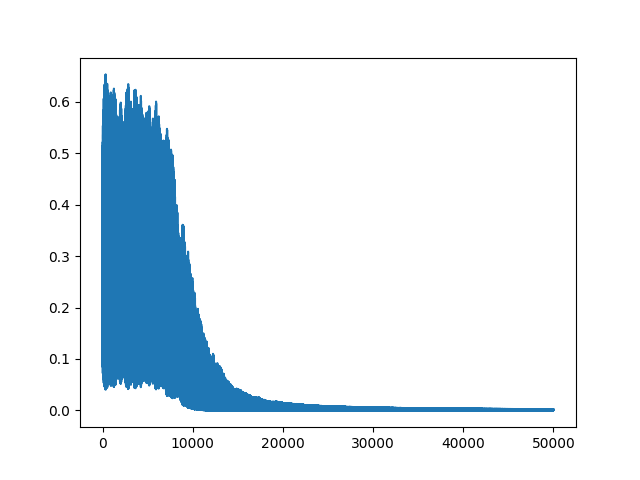
\includegraphics[width=\linewidth]{loss.png}
    \caption{\textbf{\texttt{loss.jpg}}}
    \end{subfigure}
    \label{fig:2}
\end{figure}



\section{Question 2}
How does the algorithm relate to the brain? For example, which brain areas might implement it, and/or which neural circuits? Does it explain particular data observed in neuroscience?\\

Answer2:\\
Supervised learning is woking at cerebellum part of the brain and backpropagation network it is belongs to supervised learning.
Therefore, backpropagation network is work in cerebellum.\\
It is proved that biology phenomenon know as action potential backpropagation is not directly relate to backpropagation.\\
There are some 6 key reasons to prove that backpropagation seems not to be biologically plausible. Weight transport problem, Derivative of activation functions, two phase learning, target, seperate error network, non-local learning rule.\\
First, target it is very difficult to generate the target signal in our brain \\
Second, there is no evidence prove that the weight of the feedforware and feedback would be queal.\\
Third, in biology it is not clear enough how each neurons can calculate it's derivative so this cause derivative of activation probelm.\\
Forth, in brain there is no obvious line to seperate preception and learning so two phase learning problem comes out.\\
Fifth, we use chain rule to seperate error network however there is no enough evidece to prove it.\\
Finally, in brain synapses can access local information however backpropagation is not.\\
Fortunately, two phase learning, seperate error network and non-local learning rule problems can be solved(Guerguiev et al.)\\



\section{Question 3}
What are its key advantages over the other two learning algorithms/paradigms?\\

Answer3:\\
Supervised learning is easier to understand and interpret results if we choose the correct assumptions or prior the model it would be better than unsupervised learning\\
On the other hand, unsupervised learning is capable of fitting a large number of functional forms cause it has no assumptions (or weak assumptions) about the underlying functions, as well as it can result in higher performance models for prediction.\\
Backpropagation algorithm is suitable in classification however sparse coding is suitable in computer vision and image recognition.\\



\section{Question 4}
What about disadvantages? And how could this be improved upon?\\

Answer4:\\
The disadvantage of supervised learning is that it is highly constrained to the specified functional form we choose and it is more suited to simpler problems. \\
The disadbantages of backpropagation are local minima and slow convergence(Gori, Tesi 1992).\\
Local minima problem is usually caused by update not smoothly between weights connected to the hidden layer and the output layer.\\
Slow convergence.\\
However it still have some solutions to avoid this disadvantage. For example modified error function (BI et al.)\\
In biological part supervised learning need a target however however how the brain get the teaching signal is a problem.\\
Using backpropagation algorithm is very easy to train a model which cotains input and output but it is very difficult to recognize lots of things than other network such as sparse coding.\\








References:\\
1. Avoiding the Local Minima Problem in Backpropagation Algorithm with Modified Error
Function (BI et al. 2005)
2. Magoulas , F. D., Vrahatis, M. N., AAnfroulakis, G. S.(1999) Improving the convergence of the backpropagation algorithm using learning rate adaption methods. Neural comptation, 11(7), 1769-1796





\end{document}